\documentclass[british]{beamer}

\usepackage{default}
\usepackage[british]{babel}
\usepackage{epstopdf}
\usetheme{Madrid}
\usepackage{graphicx}
\usepackage{dirtytalk}
\usepackage{csquotes}
\usepackage{wrapfig}
\usepackage{tikz}
\usepackage{smartdiagram}

\begin{document}
%
\title[Document Semantic Similarity]
{Document Semantic Similarity}

\subtitle{TIS Project}

\author[A. Pirovano, F. Picciotti]
{Alberto Pirovano \and Francesco Picciotti}

\institute[PoliMi]
{
	Politecnico di Milano
}

\logo{
	\includegraphics[height=1.7cm,trim={0 2cm 4.5cm 2cm},clip]
	{./Imgs/Politecnico-di-Milano-3-m8qw.eps}
	}	

\AtBeginSection[]
{
	\begin{frame}
		\frametitle{Outline}
		\tableofcontents[currentsection, currentsubsection]
	\end{frame}
}

\AtBeginSubsection[]{
	\begin{frame}
		\frametitle{Outline}
		\tableofcontents[currentsection, currentsubsection]
	\end{frame}
}

\maketitle

\section{State of art}

\begin{frame}{Introduzione}
	Le tecniche adottate attualmente per trovare la \textbf{similitudine semantica tra testi} si basano su tre approcci:
	\begin{enumerate}
		\item NLP Tradizionale
		\item Vector Space Model
		\item Deep Learning based 
	\end{enumerate}
\end{frame}
	
\subsection{NLP tradizionale}
	
\begin{frame}{NLP Tradizionale}
	Questo approccio si basa sull'utilizzo delle tradizionali tecniche di \textbf{Natural Language Processing} e si costituisce dei seguenti step:
	\begin{itemize}
		\item Cleaning dei dati
		\item Pos-Tagging
		\item Stemming o Lemmatisation
		\item Parsing
		\item Ontologia
	\end{itemize}
	Tuttavia, dato che il nostro lavoro \`{e} molto \textbf{sensibile} e \textbf{dipendente} dalla qualit\`{a} dei tool utilizzati, abbiamo trovato alcune consistenti \textbf{criticit\`{a}} riguardanti:
	\begin{itemize}
		\item \textbf{L'affidabilit\`{a}} del Pos-Tagger italiano di TreeTagger
		\item \textbf{Reperire} una Ontologia e un parsing toll per la  lingua italiana
	\end{itemize}
\end{frame}

\begin{frame}{NLP Tradizionale}
	\includegraphics[width=0.9\textwidth, height=0.85\textheight]{./Imgs/nlp-the-process.jpg}
\end{frame}
	
\subsection{Vector Space Model}
	
\begin{frame}{Vector Space Model}
	\begin{wrapfigure}{r}{0.4\textwidth}
		\includegraphics[width=1.1\linewidth,height=0.4\textwidth]{./Imgs/vector_space.png}
	\end{wrapfigure}	
	Differentemente dal precedente, questo approccio ha le sue basi nello sviluppo di una \textbf{rappresentazione geometrica e vettoriale} delle parole o dei documenti. Nel primo caso si parla di analisi \textbf{word-level} e nel secondo di \textbf{document-level}.
	
	Gli elementi testuali che si vogliono analizzare sono rappresentati in uno \textbf{spazio vettoriale}, le quali \textbf{dimensioni} sono gli elementi di un dizionario.
	
	Se l'obbiettivo \`{e} generare un \textbf{modello fine grained word level}, le dimensioni sono le parole del \textbf{Bag of Word} ottenuto da tutti i documenti.
\end{frame}

\begin{frame}{Vector Space Model}
	Questo approccio si articola nei seguenti \textbf{passaggi}:
	\begin{itemize}
		\item Cleaning dei dati
		\item Stemming o Lemmatisation
		\item Document/word encoding
		\item TF/IDF + LSA (Latent Semantic Analysis)
		\item Similarity (Cosine, Pearson, ...)
	\end{itemize}
\end{frame}
	
\begin{frame}{...limiti?}
	\includegraphics[width=0.9\textwidth, height=0.8\textheight]{./Imgs/bow-example.jpeg}
\end{frame}
	
\begin{frame}{Geometrico: limiti}
	Per riassumere:
	\begin{itemize}
		\item \textbf{Molto dipendente dal preprocessing del corpus}
		\item Grande Bag Of World $\rightarrow$ bisogno di LSA, ma non \`{e} cos\`{i} banale.
		
		Perch\'{e}?
		\begin{displayquote}
			"LSA assumes that words that are close in meaning will occur in similar pieces of text"
		\end{displayquote}
		\item Semantica e ambiguit\`{a}
		\item Un documento \`{e} un insieme \alert{non ordinato} di parole  
	\end{itemize}
\end{frame}
	
\subsection{Deep Learning}
	
\begin{frame}{E non solo}
	\begin{figure}[!hf]
		\centering
		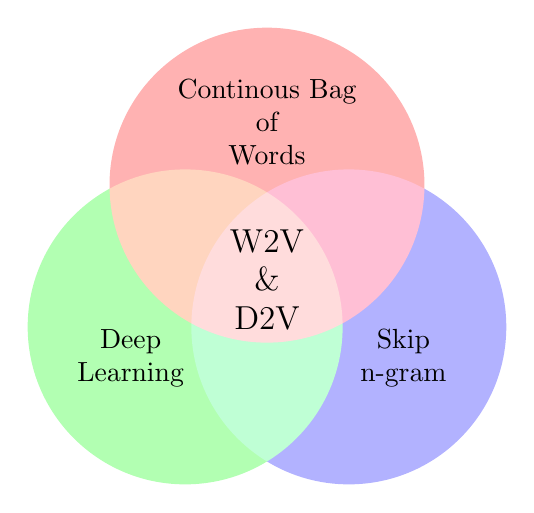
\begin{tikzpicture}
		\begin{scope}[blend group = soft light]
		\fill[red!30!white]   ( 90:1.2) circle (2);
		\fill[green!30!white] (210:1.2) circle (2);
		\fill[blue!30!white]  (330:1.2) circle (2);
		\end{scope}
		\node at ( 90:2)    
		[font= \normalsize, align= center]
		{Continous Bag \\ of \\ Words};
		\node at ( 210:2)   
		[font= \normalsize, align= center]
		{Deep \\ Learning};
		\node at ( 330:2)   
		[font= \normalsize, align= center]
		{Skip \\ n-gram};
		\node [font=\large, , align= center] {W2V \\\& \\D2V};
		\end{tikzpicture}
	\end{figure}
\end{frame}
	
\begin{frame}{Deep Learning: W2V \& D2V}
	Negli ultimi anni il \textbf{Deep Learning} \`{e} stato usato in numerosi ambiti con ottimi risultati.\par
	In particolare \textbf{Google}, con la release di \textbf{Word2Vec}, ha offerto alla community una tecnica per determinare \textbf{la similarit\`{a} semantica} che un particolare \textbf{corpus di testi} assegna ad un \textbf{Bag Of Words} di parole.
	\textbf{Doc2Vec} invece, rilasciato anche esso da \textbf{Google}, \`{e} una tecnica che si configura come una \textbf{estensione di Word2Vec} che, preso in ingresso un set di documenti (corpora), genera un \textbf{grado di similarit\`{a}} reciproco.
\end{frame}

\begin{frame}{Pros and Cons}
	Dopo una ampia \textbf{discussione}, seguita da una approfondita \textbf{analisi critica} di questi due approcci, siamo giunti alle seguenti \textbf{conclusioni}, che in termini di pro e contro si possono riassumere nel seguente modo:
	\begin{columns}
		\column{0.5\textwidth}
		\\
		\underline{Pros:}
		\begin{itemize}
			\item Molto meno dipente da un preprocessing
			\item \textbf{Context-aware}
			\item Combina il metodo \textit{Geometrico} con quello \textit{NLP Tradizionale}
			\item \textbf{Non sfrutta una ontologia, ma la \alert{crea}} 
		\end{itemize}
		\column{0.5\textwidth}
		\underline{Cons:}
		\begin{itemize}
			\item Tecnica \textbf{unsupervised}
			\item Necessit\`{a} di un esperto per \textbf{validare} la similarit\`{a}
			\item Pu\`{o} risultare in \textbf{GIGO} system (Garbage In Garbage Out)
		\end{itemize}
	\end{columns}
\end{frame}
	
\section{Data Preparation}

\begin{frame}{Dataset}
	\begin{displayquote}
		"Preprocessing is 80\% of NLP work"
		 
		\begin{flushright}
			\textit{Lev Konstantinovskiy}
		\end{flushright}
	\end{displayquote}
	Il dataset fornitoci \`{e} composto da due corpora: 
	\begin{itemize}
		\item il corpus del Sole 24 Ore con 3265 articoli, di cui 31 non hanno body
		\item il corpus di Radiocor con 6916 articoli
	\end{itemize}
	Il corpus prima del preprocessing contiene quindi 10150 articoli. \par
	Togliendo i duplicati otteniamo 9283 articoli, cio\'{e} ci sono 867 articoli duplicati.
\end{frame}

\subsection{Preprocessing}

\begin{frame}{Pipeline completa}
	\begin{center}
		\smartdiagramset{
			module minimum width= 5cm, 
			text width= 4.5cm,
			font= \tiny,
			set color list={blue!50!cyan,green!60!lime,orange!50!red,red!80!black},
			back arrow disabled=true}
		\smartdiagram[flow diagram: horizontal]{Cleaning del testo,Tokenizzazione e rimozione punteggiatura, Rimozione stopwords e POS-tagging del testo,Lemmatizzatione,Merge di verbi passivi composti}
	\end{center}
\end{frame}

\subsection{Cleaning del testo}

\begin{frame}{Cleaning pipeline}
	\begin{center}
			\smartdiagramset{
				module minimum width= 5cm,
				module minimum height= 0.1cm, 
				text width= 5cm,
				module y sep= 0.8cm,
				font= \tiny,
				set color list={blue!50!cyan,green!60!lime,orange!50!red,red!80!black},
				back arrow disabled=true}		
			\smartdiagram[flow diagram: vertical]{Lowercase di ogni lettera, Escape di caratteri unicode non printabli, Tokenizzazione numeri percentuali, Rimozione preposizioni contratte, Tokenizzazione parola s24, Unificazione di espressioni di quantit\`{a}, Rimozione di intestazione di articolo, Rimozione di interruzione pagina, Rimozione chiusura aricolo, Rimozione urls e tags html}
	\end{center}
\end{frame}

\section{Word2Vec}

\begin{frame}{Hello}
	Qui speghiamo per bene come funziona word2vec
\end{frame}

\section{Doc2Vec}

\begin{frame}{Hello}
	Qui speghiamo per bene come funziona word2vec
\end{frame}
\end{document}
